\documentclass{scrartcl}

% packages
\usepackage{amsmath}
\usepackage{amssymb}
\usepackage[ngerman]{babel}
\usepackage{booktabs}
\usepackage[font=small,labelfont=bf]{caption}
\usepackage{csquotes}
\usepackage{float}
\usepackage{fontspec}
  \setmainfont[Ligatures=TeX]{Tex Gyre Pagella}
\usepackage{graphicx}
\usepackage[pdfusetitle,unicode]{hyperref}
\usepackage{mathtools}
\usepackage{microtype}
\usepackage{siunitx}
  \sisetup{separate-uncertainty=true}
\usepackage{subcaption}
\usepackage[math-style=ISO,bold-style=ISO]{unicode-math}
  \setmathfont{Tex Gyre Pagella Math}
\usepackage{xfrac}

% options
\setlength{\parindent}{0pt}  % no stupid indentation

% commands
\DeclarePairedDelimiter{\abs}{\lvert}{\rvert}
\DeclarePairedDelimiter{\mean}{\langle}{\rangle}
\renewcommand{\vec}[1]{\mathbf{#1}}
\renewcommand{\i}{\mathrm{i}}
\DeclareRobustCommand{\e}{\ensuremath{\mathrm{e}}}

% meta
\author{Kevin Dungs \and Kevin Heinicke \and Holger Stevens}
\title{Computational Physics}
\subtitle{Übungsblatt 3}

% document
\begin{document}
\maketitle

\section*{Hausaufgabe 7: Testen von Zufallsgeneratoren}
\paragraph{a) - d)} In der Klasse \texttt{Randinium.hpp} (implementierung in \texttt{Randinium.cpp}) wird der angegebene Zufallszahlengenerator bereitgestellt.
Mittels \texttt{make plots} werden sowohl $10^6$ Zufallszahlen generiert und in einem Histogramm (\texttt{plots/hist.pdf}) dargestellt, als auch Punkte von Zahlenpaaren, bzw. Tripletts erzeugt und geplottet.

Schon in dem Histogramm Abb. \ref{fig:histogram} lässt sich eine Periodizität der Zahlen erkennen. Obwohl die Verteilung sehr flach ist, liegt offensichtlich keine Gleichverteilung vor.
Die Wahl des Startwertes hat hierauf keine Auswirkungen, da die Periode dieser Zahlen wesentlich kleiner ist, als die Anzahl der erzeugten Zahlen.

\begin{figure}[H]
    \centering
    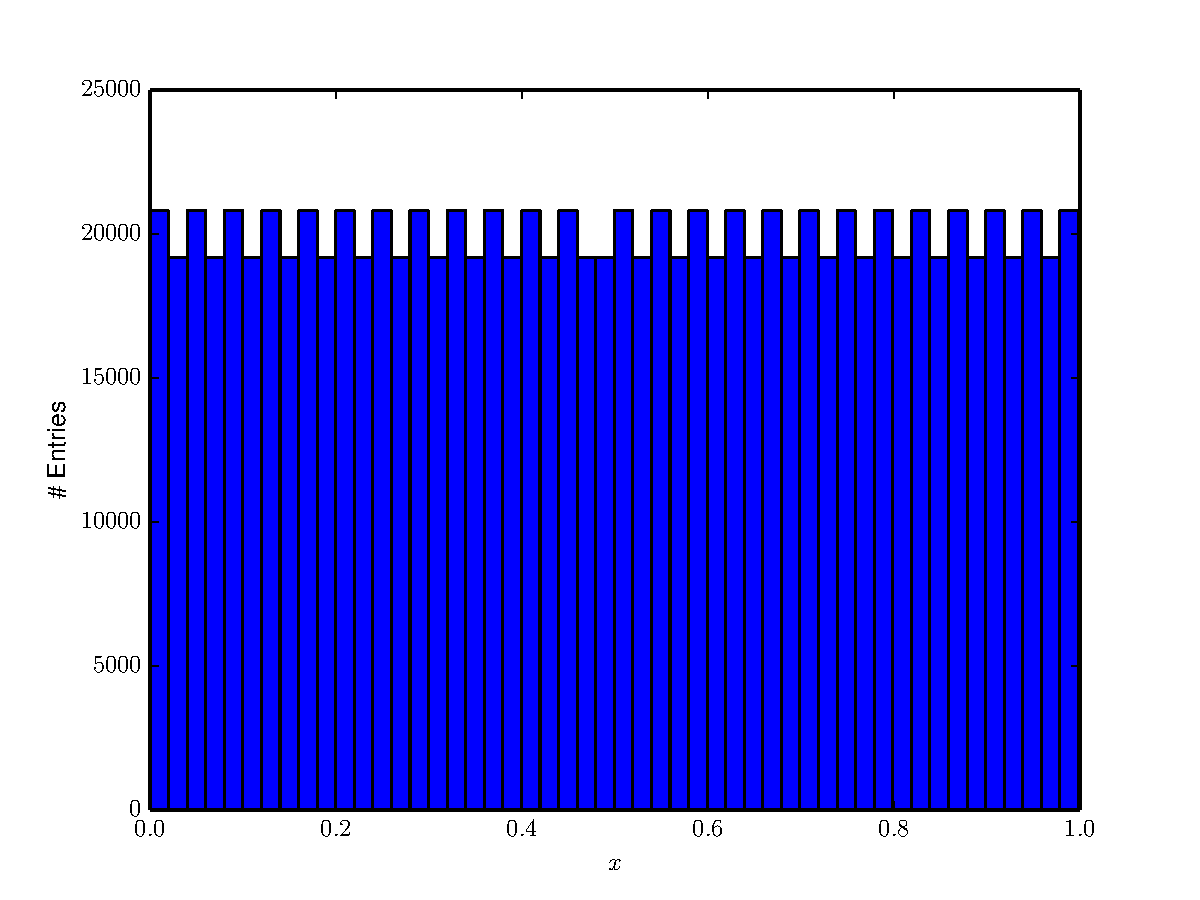
\includegraphics[width=0.5\textwidth]{plots/hist.pdf}
    \caption{Zufallszahlenverteilung aus der angegebenen Vorschrift}
    \label{fig:histogram}
\end{figure}

Zusätzlich werden die entsprechenden 2D- und 3D- Histogramme mit \texttt{rand()} und \texttt{std::mt19937} erzeugt.


Exemplatrisch sind in Abb. \ref{fig:3DLK} und \ref{fig:3DMT} zwei 3D-Plots aufgeführt. Spätestens hier wird die Periodizität der angegebenen Zufallszahlen durch die auftretenden Ebenen deutlich. Die mittels Mersenne Twister Verfahren oder \texttt{rand()} erzeugten Zahlen bieten die deutlich bessere Wahl. Weitere Plots sind im Ordner \texttt{plots/} zu finden.

\begin{figure}[H]
    \centering
    \begin{subfigure}{0.45\textwidth}
        \centering
        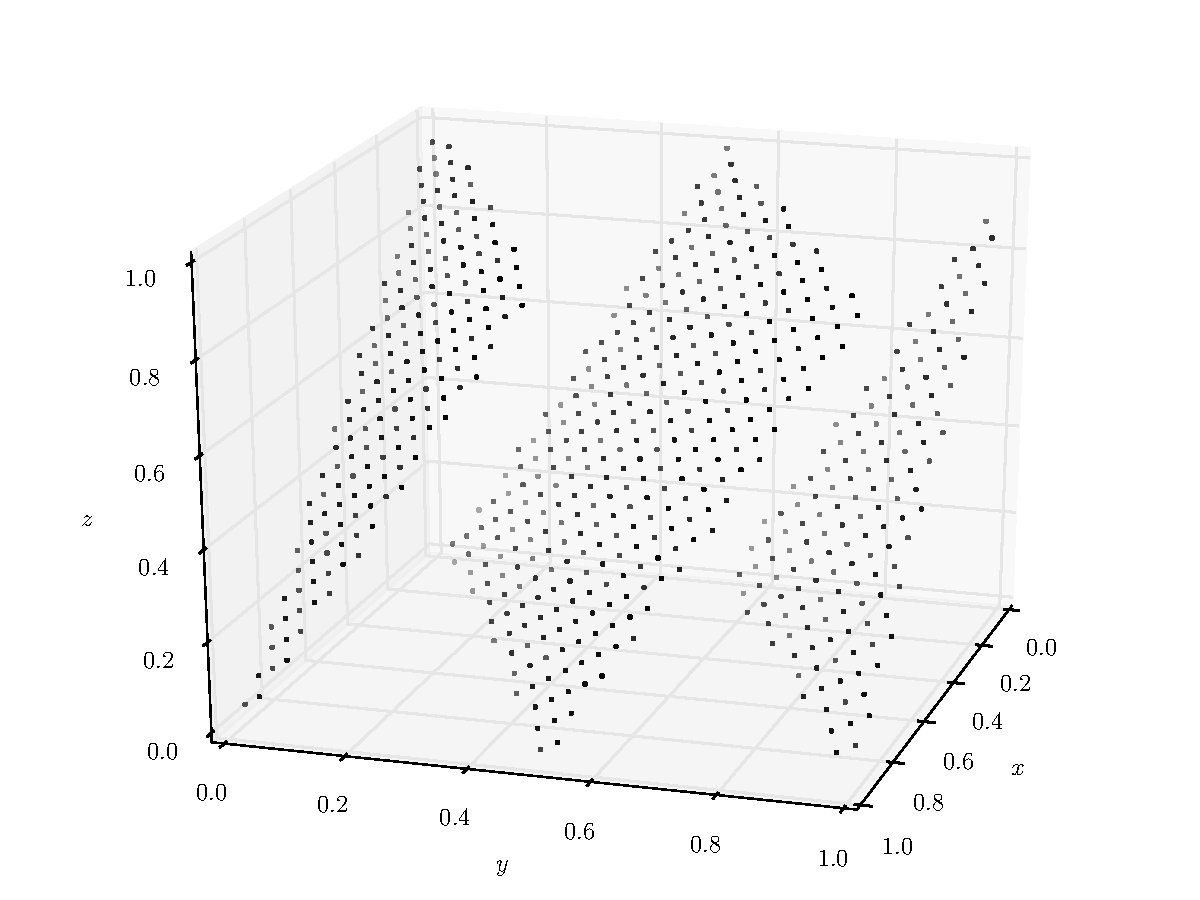
\includegraphics[width=\textwidth]{plots/dist3d.pdf}
        \caption{Zufallszahlen, erzeugt mit Hilfe des angegeben linearen Kongruenzverfahren: Eine deutliche Periodizität ist zu erkennen.}
        \label{fig:3DLK}
    \end{subfigure}
    \hfill
    \begin{subfigure}{0.45\textwidth}
        \centering
        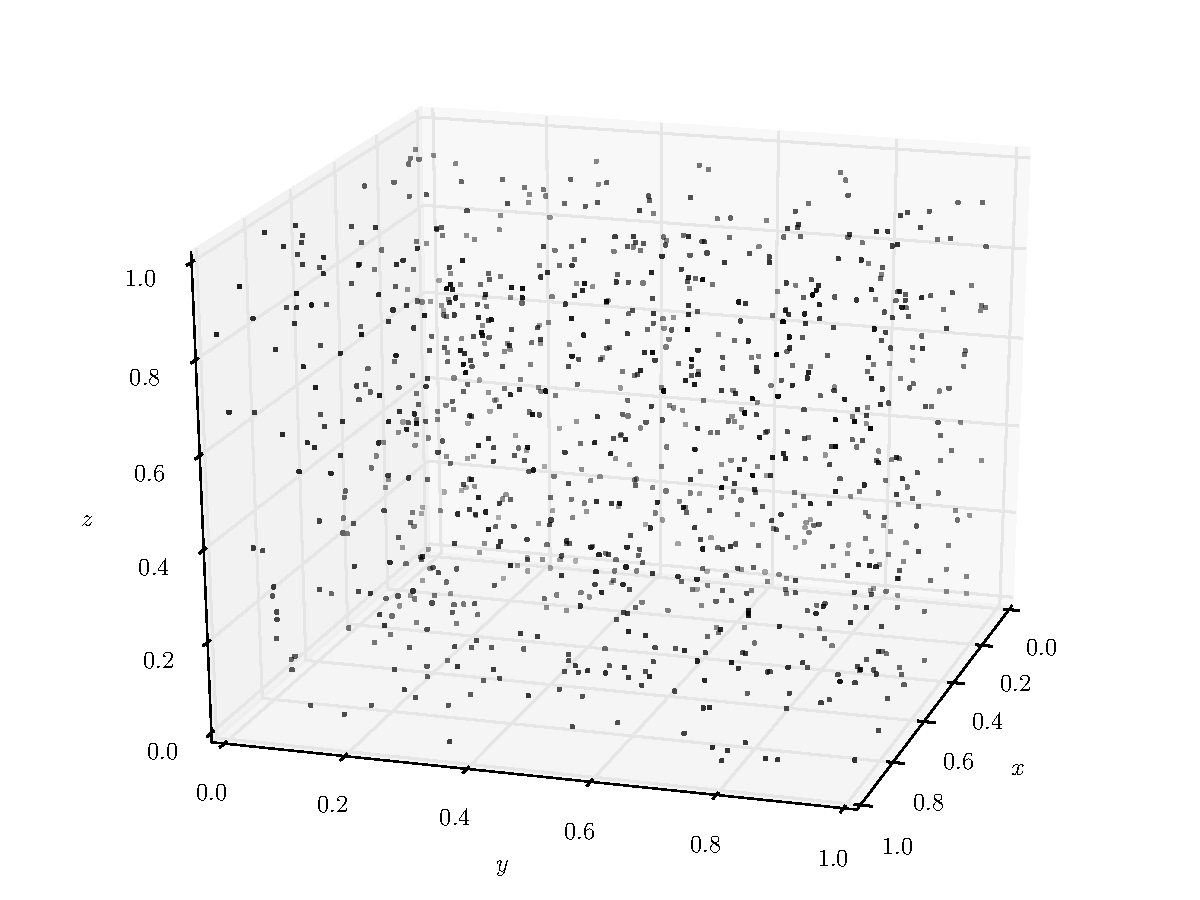
\includegraphics[width=\textwidth]{plots/dist3d_mt.pdf}
        \caption{Zufallszahlen, erzeugt mittels Mersenne Twister: Die Wolkenstruktur deutet auf Normalverteilung hin.}
        \label{fig:3DMT}
    \end{subfigure}
\end{figure}

\section*{Hausaufgabe 8: Beliebige Verteilungen erzeugen}
Alle Implementierungen basieren auf Konzepten in C++11. Informationen zum Konzept der Zufallsverteilungen finden sich auf \url{http://en.cppreference.com/w/cpp/concept/RandomNumberDistribution}. Für die Aufgabenteile (a) und (b) wurde das Konzept vollständig implementiert. Bei den anderen Aufgaben wurde aus Zeitgründen darauf verzichtet und nur die Kernfunktionalität umgesetzt.

\paragraph{(a, b)} Die Implementierungen finden sich in \texttt{boxmueller.hpp} und \texttt{centrallimit.hpp}. Mit Hilfe von \texttt{distributions.cc} werden jeweils \num{1e5} Zufallszahlen erzeugt und mit \texttt{hists.py} geplottet. Das Ergebnis ist in \autoref{fig:gaussian} zu sehen. Obwohl die Implementierungen beliebige Mittelwerte und Breiten der Verteilungen erlauben, wird hier die Standardnormalverteilung ($\mu = 0, \sigma = 1$) verwendet.

Für den Mittelwert von $N$ Zufallszahlen $S_N$, deren Verteilung den Erwartungswert $\mathrm{E}[x] = \mu$ und die Varianz $\mathrm{Var}[x] = \sigma^2$ hat, gilt im Limes $N \to \infty$
\begin{equation}
    \sqrt{N}(S_N - \mu) \sim \mathcal{N}(0, \sigma^2)
\end{equation}
wobei $\mathcal{N}$ die Normalverteilung ist. Um also mit Hilfe des zentralen Grenzwertsatzes aus $N$ gleichverteilten Zufallszahlen $x_i$ im Bereich $[0, 1)$ eine Standardnormalverteilung zu approximieren, wird der Mittelwert der $x_i$ berechnet, davon der Mittelwert der Verteilung (hier $\mu = \num{.5}$) abgezogen und das Ergebnis mit $\sqrt{12N}$ multipliziert. Die $12$ ergibt sich aus der Varianz der Gleichverteilung ($\sigma^2 = \sfrac{1}{12}(1 - 0)^2$).

\begin{figure}[H]
    \centering
    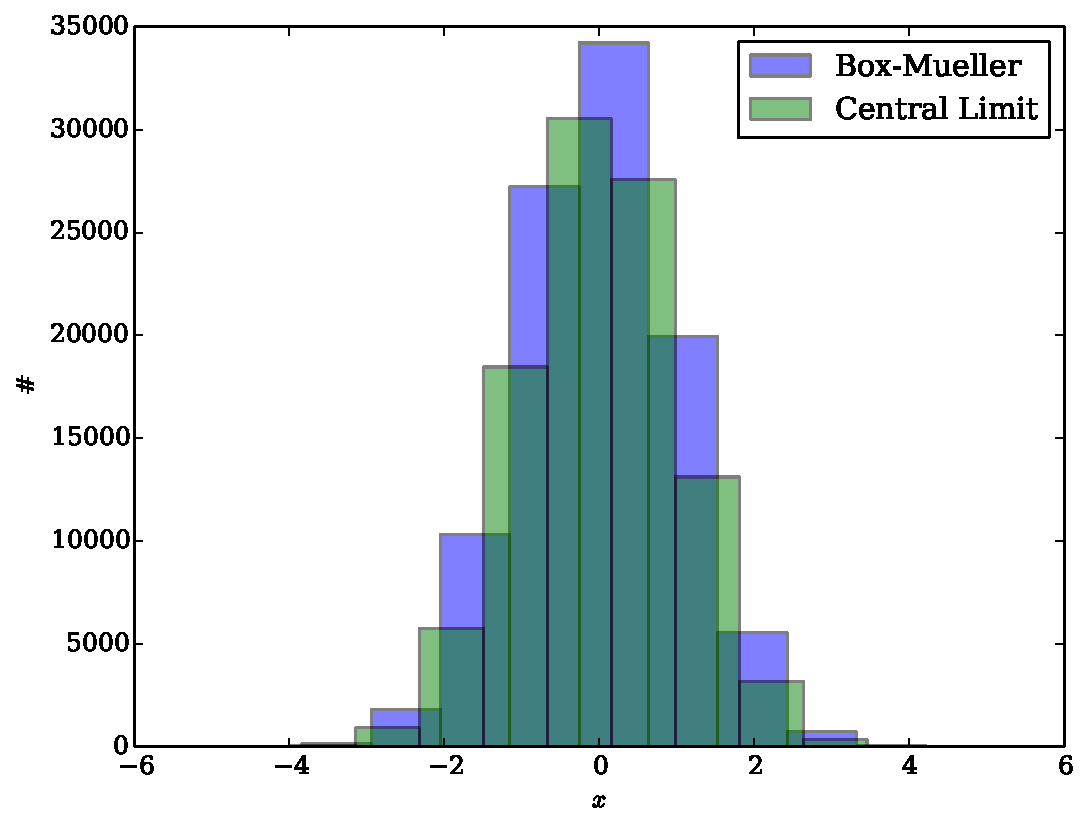
\includegraphics[width=.5\textwidth]{plots/gaussian.pdf}
    \caption{Standardnormalverteilungen aus verschiedenen Methoden.}
    \label{fig:gaussian}
\end{figure}

\paragraph{(c)} Die Lösung der Aufgabe ist in \texttt{acceptreject.hpp} zu finden. Auch hier werden mit \texttt{distributions.cc} \num{1e5} Zufallszahlen erzeugt und mit \texttt{hists.py} geplottet. Das Ergebnis ist in \autoref{fig:sinxover2} zu sehen.

\begin{figure}[H]
    \centering
    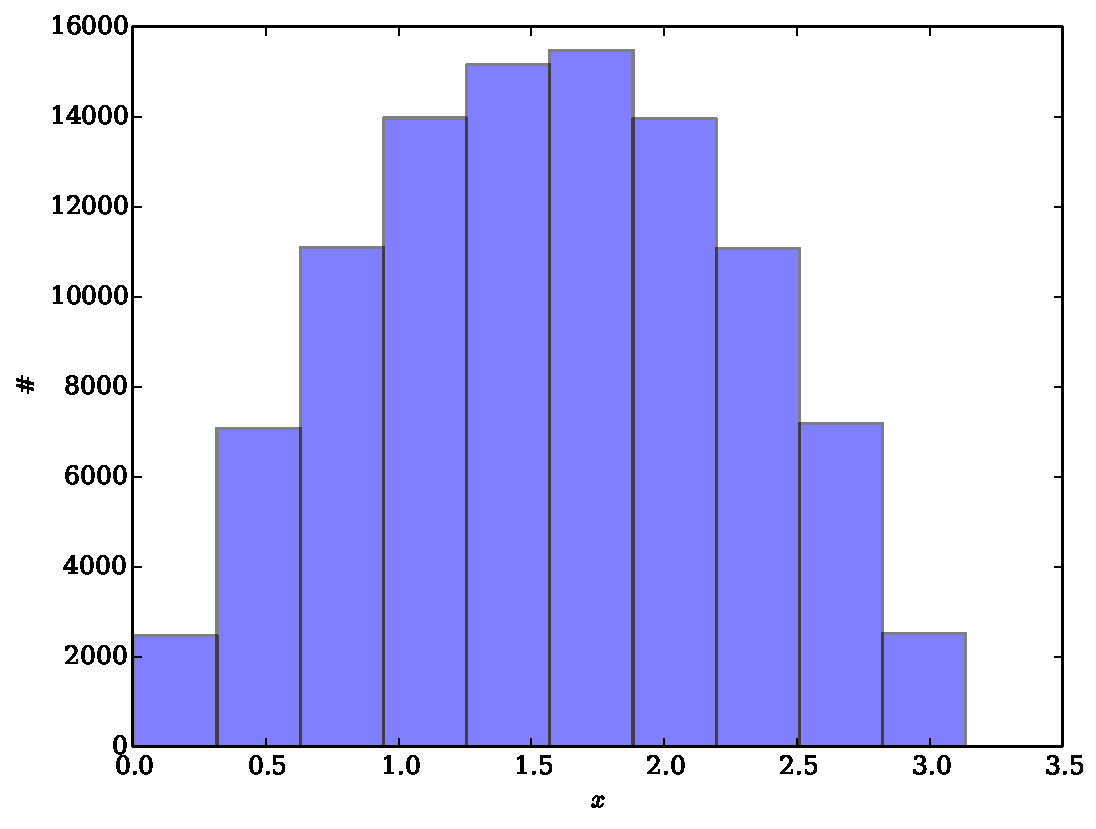
\includegraphics[width=.5\textwidth]{plots/sinxover2.pdf}
    \caption{Zufallszahlen deren Verteilung $\sin(x)/2$ entspricht.}
    \label{fig:sinxover2}
\end{figure}

\paragraph{(d)} Zunächst muss aus der PDF $f(x) = 3x^2$ die CDF $F(x)$ berechnet werden:
\begin{equation}
    F(x) = \int_0^x\mathrm{d}t\,f(t) = \left[t^3\right]_0^x = x^3
\end{equation}
Als Inverse dieser Funktion ergibt sich
\begin{equation}
    F^{-1}(x) = \sqrt[3]{x}
\end{equation}
Die Implementierung ist in \texttt{transformation.hpp} zu finden. In \autoref{fig:3xsquared} ist das Ergebnis der Erzeugung von \num{1e5} Zufallszahlen zu sehen.

\begin{figure}[H]
    \centering
    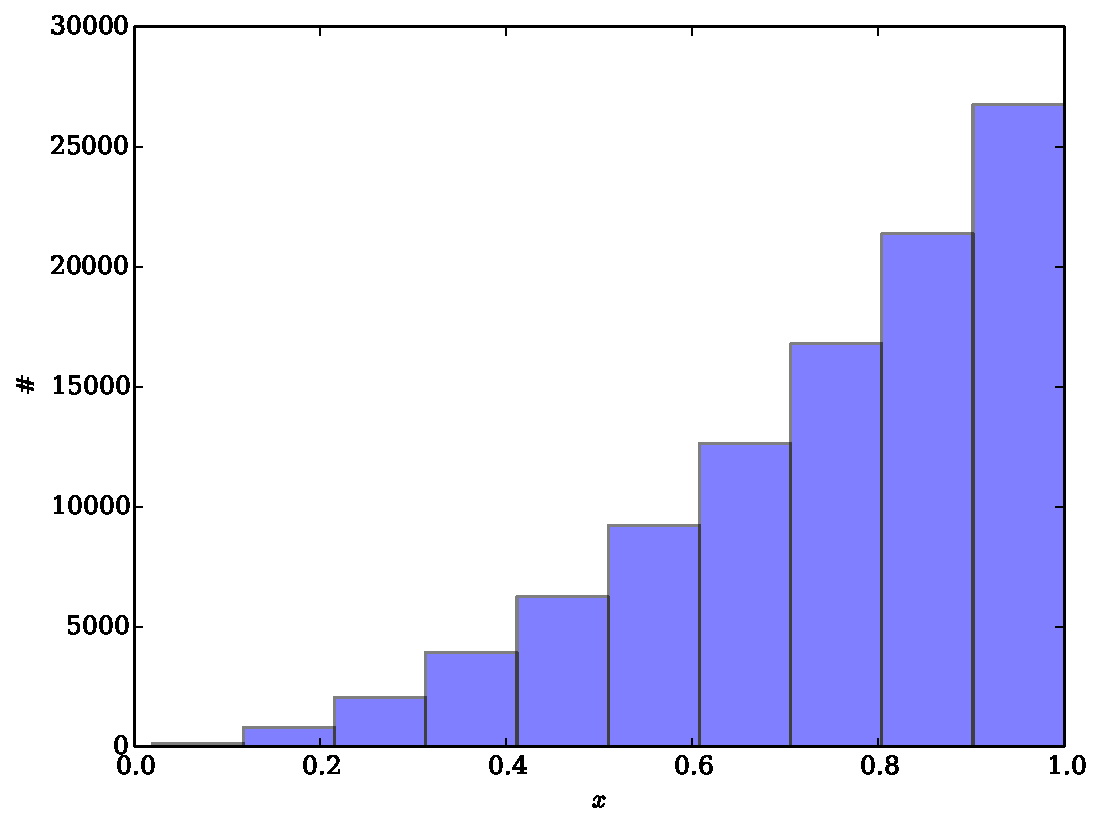
\includegraphics[width=.5\textwidth]{plots/3xsquared.pdf}
    \caption{Zufallszahlen deren Verteilung $3x^2$ entspricht.}
    \label{fig:3xsquared}
\end{figure}

\end{document}
